%!TEX root = paper.tex
Until now, our analysis has assumed that in order to find a torrent and begin the download process a node must directly identify a node currently participating in that torrent. This need not be the case. Rather, to find a torrent, we could first discover the torrent's tracking data. The tracking data will contain a list of nodes thought to be participating in the torrent, and these nodes can be used to initiate the download. This is, of course, analogous to the original BitTorrent protocol's torrent-discovery-via-trackers mechanism. To accomplish this in a unstructured P2P environment, we need a mechanism by which each peer indexes a random, non-disjoint subset of torrent tracking data. Given this mechanism, we can apply PAC search on the collection of tracking data, where each torrent's tracking data is equivalent to a document. The success of PAC search is then dependent on the distribution of torrent tracking data, rather than the distribution of the torrents themselves. 

In Section~\ref{sec:extension:indexing} we first introduce the modification to the BitTorrent protocol that enables peers to index a random, non-disjoint subset of torrent tracking data. Section~\ref{sec:extension:model} provides a mathematical model of our extension. Section~\ref{sec:extension:discussion} then analyses the distribution of torrent tracking data and the associated performance of PAC search.

\subsection{Indexing}\label{sec:extension:indexing}

    Our modification is based on the following assumptions, which are discussed shortly. First, we assume that a querying node is able to sample and communicate with $z$ random nodes in the network. This is a key assumption behind the PAC search framework. Second, we assume that a querying node will persist in communicating with nodes until the search is successful, i.e. the querying node identifies a node that is either participating in the torrent or is indexing a node participating in the torrent. Thus, when a node performs a {\em search} it issues one or more queries for the same torrent, until such time as a query is successful. A {\em query} consists of a node sending a request to $z$ randomly sampled nodes in the network. Each repeated query for the same torrent selects $z$ different nodes. A {\em request} consists of a querying node sending the desired torrent's infohash to a random node. The queried node responds with either a list of nodes it believes are participating in the torrent, or an empty list.

    When a node receives a query, it updates its index, such that the querying node is now added to the requested torrent's list of participating nodes. If the index does not already contain a record for the torrent, a new record is inserted with the querying node listed as a participating node. In this way, a queried node builds up a local database of tracking data.

    In the next section, we analyse the expected distribution of tracking data across nodes and show that this distribution is capable of supporting PAC search.

\subsection{Model}\label{sec:extension:model}

    When querying a fixed number of random nodes, $z$, the probability of a successful query is now determined by (i) the number of nodes participating in the torrent, and (ii) the number of nodes indexing the torrent's tracking data, $r_i$. Given our proposed modification to the BitTorrent protocol, the more queries the network receives for a torrent, the more that torrent's tracking data is replicated, and the easier it becomes to find. The number, $r(t)$, of nodes indexing a torrent at a time $t$ depends on: the number, $u$, of requests made for the torrent at $t$, and the proportion, $c$, of nodes that leave the network at $t$. The change in replication over time can be expressed as:

    \begin{equation}
        \frac{dr(t)}{dt} = u(1+z(1-\frac{r(t)}{n}))-cr(t)
        \label{eq:drdt}
    \end{equation}

    Here, $1-\frac{r(t)}{n}$ gives the proportion of the $z$ nodes that were not already indexing the torrent. We can solve this ODE to give us an equation for the replication as a function of time:

    \begin{equation}
        r(t) = ke^{-t(c+\frac{uz}{n})}+\frac{un(1+z)}{uz+cn}
        \label{eq:rt}
    \end{equation}

    The constant, $k$, is given by the initial condition, $r(0)$. Conceptually, $r(0)$ is the number of nodes that index the torrent before any queries have been made for it. The torrent's author can control $r(0)$ in order to enable early queries to be successful. The authoring node simply makes dummy requests to $r(0)$ nodes in order to push tracking data into the network.

\subsection{Discussion}\label{sec:extension:discussion}

    Eqn~\ref{eq:rt} gives the replication of a torrent's tracking data as a function of time. It depends on a number of constants; $c$, the network churn rate, $u$ the torrent query rate, $z$ the query size, and $n$ the network size. We see that $r(t)$ approaches a limit of $\frac{un(1+z)}{uz+cn}$ at an exponential rate. After some small $t$, therefore, we can consider $r(t)$ to be stable, with negligible deviation from the limit. In this steady state condition, the replication is controlled by $u$, $n$, $z$ and $c$. Both $n$ and $c$ are constants defined by the network and so are not controllable. It is possible to control $z$. In this discussion we assume a value of $z=100$. This value could be decided globally and apply to all torrents, or perhaps a dynamic value of $z$ could be picked by the torrent author or querying node. The effects and ramifications of when to pick $z$ and who gets to pick it are left for future work. The number of queries performed for the torrent, $u$, depends on the number of nodes searching for the torrent. It is also possible for participating nodes to issue dummy queries, as the authoring node does at $t=0$. In this way the query rate can also be controlled.

    In the following discussion we assume $n=5000000$. We set the churn rate c=0.06, i.e. 6\% of nodes leave the network every hour and the same number of fresh nodes enter the network. This value is based on \cite{Guo2007,Izal2004}, where the authors estimate that the average time it takes a node to download a torrent is 8.06 hours and the average time a node spends seeding that torrent is 8.42 hours. If nodes spend an average of 16.48 hours in the network then we expect $\frac{1}{16.48}=6\%$ of the network to leave every hour. This does not account for nodes that download multiple torrents and so may be an over estimate. If a torrent receives $u=100$ queries per hour then Eqn~\ref{eq:prob_find_non_uniform_distribution} tells us that $P(d_i)=0.96$ when $z=100$, thus any torrents that are receiving at least 100 queries per hour will have 96\% of the queries performed for it succeed if queries go to 100 nodes. Any query that fails can be repeated with a different set of 100 nodes and so in practise it is unlikely that any search will fail. If we decrease $u=50$ then $P(d_i)=0.81$, decreasing $z=50$ instead gives $P(d_i)=0.57$. We see that the probability of a successful query is much more sensitive to $z$ than $u$. For this reason it is important that a suitable value for $z$ is picked. Note that even when $P(d_i)=0.57$ the expected number of reepated queries required before success is only 1.75. Figure~\ref{fig:query_rate_vs_query_size} shows the relationship between $z$ and $u$ for three different values of $P(d_i)=0.5,0.7,0.9$. We conclude that even if the desired probability of a successful query were high, e.g. $P(d_i)=0.9$, that reasonable strategies for $z$ and $u$ can be picked. If the torrent is popular then low values of $z$ will still provide the probability required. If the torrent is not popular, as the majority of the torrents we observed were, then high probabilities can still be achieved by either setting $z$ higher or by artificially increasing the number of queries performed for it. For example, if we fix $z=100$ and decide on an acceptable probability of successful query, $P(d_i)=0.9$ then Eqn~\ref{eq:prob_find_non_uniform_distribution} tells us the replication needed to meet those requirements:

    \begin{align}
        r(t)_{\textrm{required}} &= n(1-\exp^{\frac{\log(1-P(d_i))}{z}}) \label{eq:rt_required}\\
                                 &= 113814
    \end{align}

    For the same rate of churn, $c=0.06$, and number of nodes in the network, $n=5000000$, we see the replication of a torrent's tracking data, $r(t)$, tending towards at least this replication level when the query rate, $u\ge69.17$. So torrents with at least 69 queries performed for it per hour will be discoverable 90\% of the time if nodes query $z=100$ nodes at a time. In our measurement study 76\% of the torrents that we observed were available on fewer than 10 nodes. It seems unlikely, therefore, that the majority of torrents would have 69 queries being performed for them. But as the torrent spreads, this may become overwhelming. It might be worth emphasising (i) that dummy request only originate from participating nodes rather than nodes that index the torrent data. Also, participating nodes could decrease or stop issuing queries if a dummy query was successfully answered, an indication that the torrent was sufficiently replicated.

    \begin{figure}[t]
        \centering
        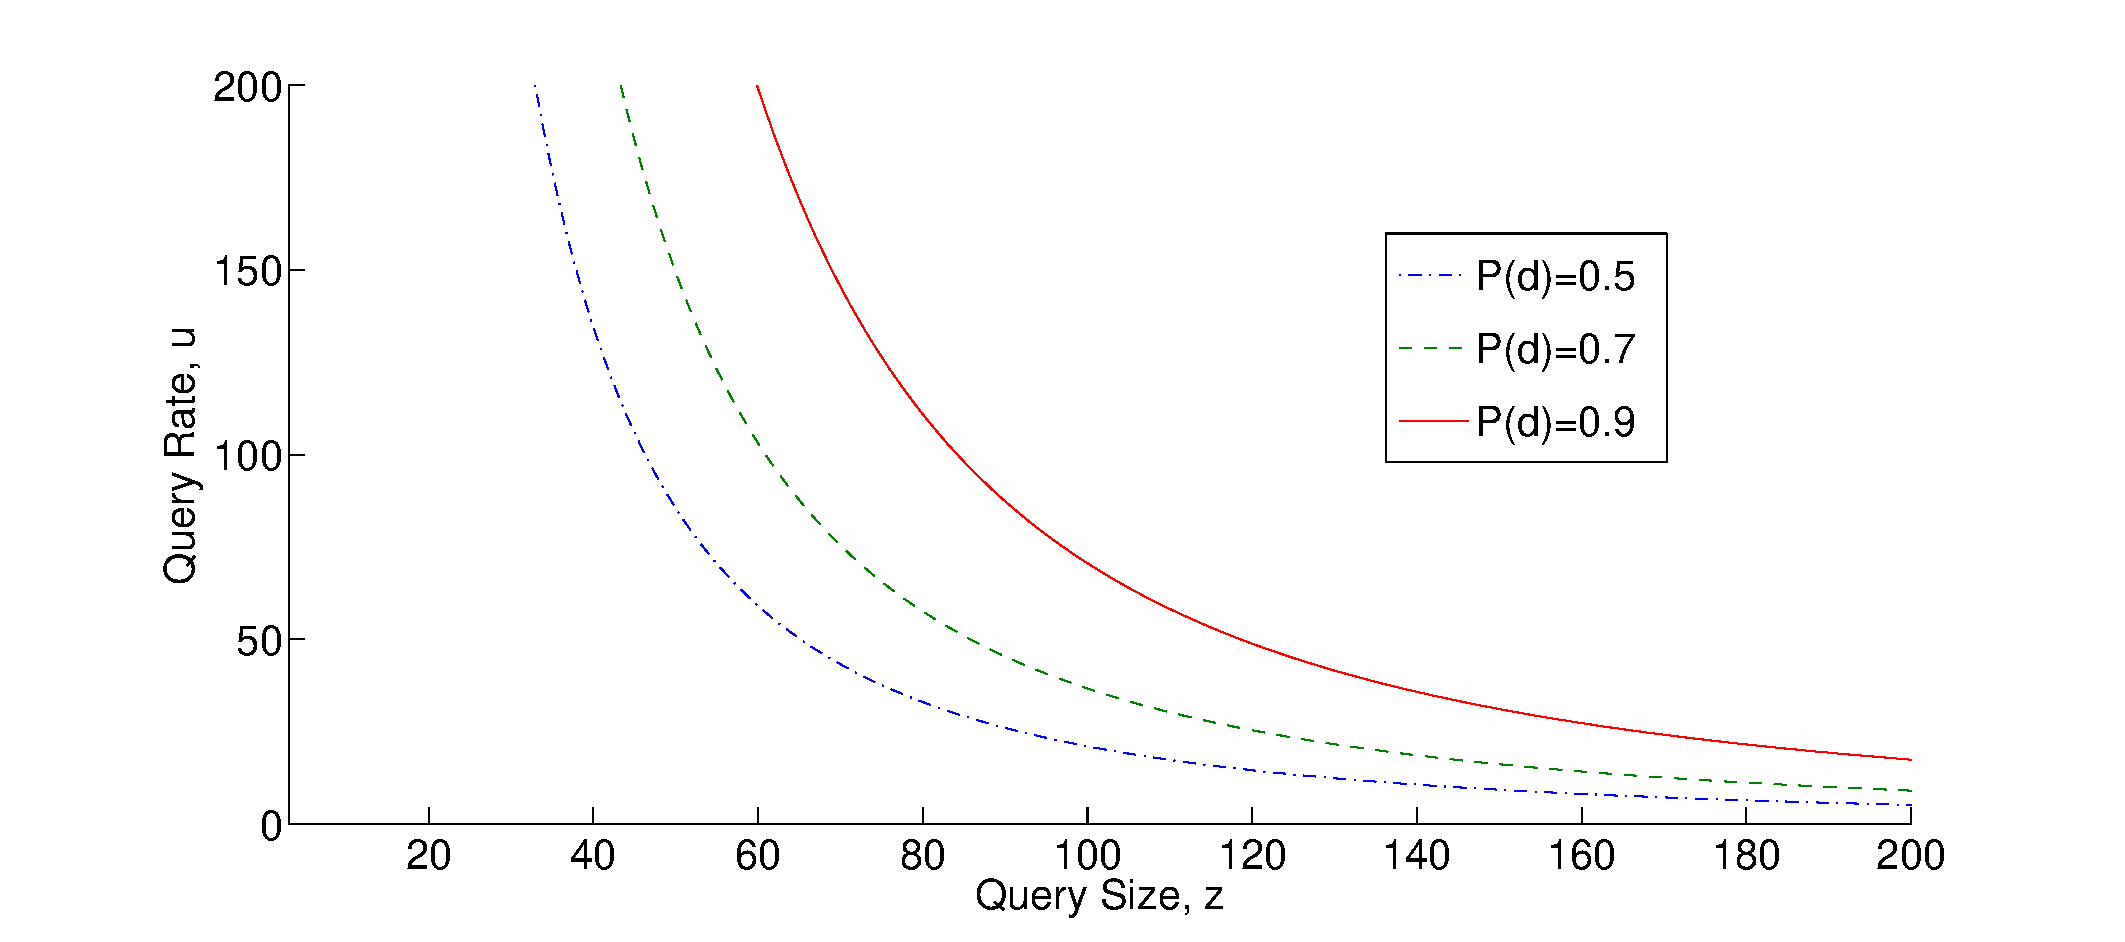
\includegraphics[width=0.5\textwidth]{Images/QueryRatevsSize.eps}
        \caption{The query rate, $u$, required to meet the probability of successful query $P(d)$ for query size, $z$.}
        \label{fig:query_rate_vs_query_size}
    \end{figure}

    The above analysis assumed that the replication had reached a stable point. As noted, this stable point is reached exponentially quickly. For small $t$ however, the replication can be very different from the steady state and therefore the probability of a successful query is also different. The value of $r(0)$ is set by the authoring node and directly controls the probability of finding the torrent in the first hour. If $r(0) > \frac{un(1+z)}{uz+cn}$ then the replication levels will be decreasing towards the limit and the probability of success will always be at or above the steady state. As seen in Eqn~\ref{eq:rt_required}, in the steady state condition the replication is high, e.g. $r(t)=113814$. It is unlikely that an authoring node would have the capacity or inclination to issue dummy queries to so many nodes. Instead the replication will be increasing towards the limit. $r(0)$ can therefore set a minimum probability of successful search. For example, if the desired minimum were $P(d_i)=10\%$, $n=5000000$, and $z=100$ then, from Eqn~\ref{eq:prob_find_non_uniform_distribution}, $r(0)=5265$. As nodes can repeat an unsuccessful query, even if the probability of any individual query is low the expected number of queries required before success can still be reasonable. For instance, with $P(d_i)=0.1$ we would expect nodes to have to query 10 times before success. After these 10 queries the replication will have increased by at most $10z$ and the probability of successful search will have increased to 12\%. Consequently, the next node to search for the torrent is expected to have to query 8.3 nodes before success. The distributing of the bootstrap tracking data can be achieved over time and so should not constitute a significant drain on the resources of the authoring node. A more in depth analysis of the overheads introduced by this extension to BitTorrent follows.
